%%%%%%%%%%%%%%%%%%%%%%%%%%%%%%%%%%%%%%%%%%%%%%%%%%
\begin{frame}[fragile]{}

\begin{center}
{
\LARGE
Why Event Sourcing?
}

\vspace{2em}

or:

\vspace{2em}

{
\Large
How this all began
}
\end{center}
\end{frame}

%%%%%%%%%%%%%%%%%%%%%%%%%%%%%%%%%%%%%%%%%%%%%%%%%%
\begin{frame}[fragile]{}

  SoCraTes Conference 2015
                  
                  11 users were incorrectly denied registration due to a bug
                  
                  We could not find out from the system who these users were
                  
                  2 or 3 complained, but the others? Gone (and probably disappointed).


\end{frame}

%%%%%%%%%%%%%%%%%%%%%%%%%%%%%%%%%%%%%%%%%%%%%%%%%%
\begin{frame}[fragile]{}

The bug: 2-phase registration (reservation -> registration)
                  
                  reservation was made, but registration was denied
                  
                  reservation token only contained session id
                  was deleted after 30 minutes
                  
                  -> we were unable to see who actually made the reservation
                  
                  How can this be improved?
                  
\end{frame}

%%%%%%%%%%%%%%%%%%%%%%%%%%%%%%%%%%%%%%%%%%%%%%%%%%
\begin{frame}[fragile]{}

\begin{center}
{
\LARGE
Event Sourcing
}

\vspace{2em}

or:

\vspace{2em}

{
\Large
Don't Drop Data!
}
\end{center}
\end{frame}

%%%%%%%%%%%%%%%%%%%%%%%%%%%%%%%%%%%%%%%%%%%%%%%%%%
\begin{frame}[fragile]{}

Usually: Relational Database
                  
                  Only captures current state!
                  
                  No information about previous states
                  No information why some change happened
                  
\end{frame}

%%%%%%%%%%%%%%%%%%%%%%%%%%%%%%%%%%%%%%%%%%%%%%%%%%
\begin{frame}[fragile]{}

How to improve this?
                  
                  Record everything that happened, and why.
                  
\end{frame}

%%%%%%%%%%%%%%%%%%%%%%%%%%%%%%%%%%%%%%%%%%%%%%%%%%
\begin{frame}[fragile]{Event Sourcing}

\begin{onlyenv}<1>
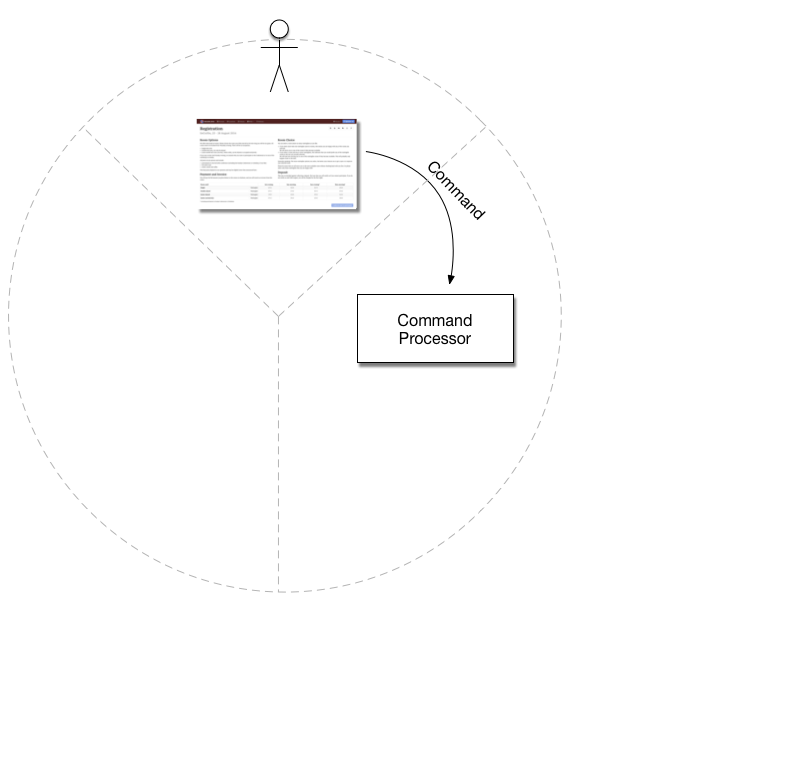
\includegraphics[width=.7\textwidth]{../EventSourcing1.png}
\end{onlyenv}

\begin{onlyenv}<2>
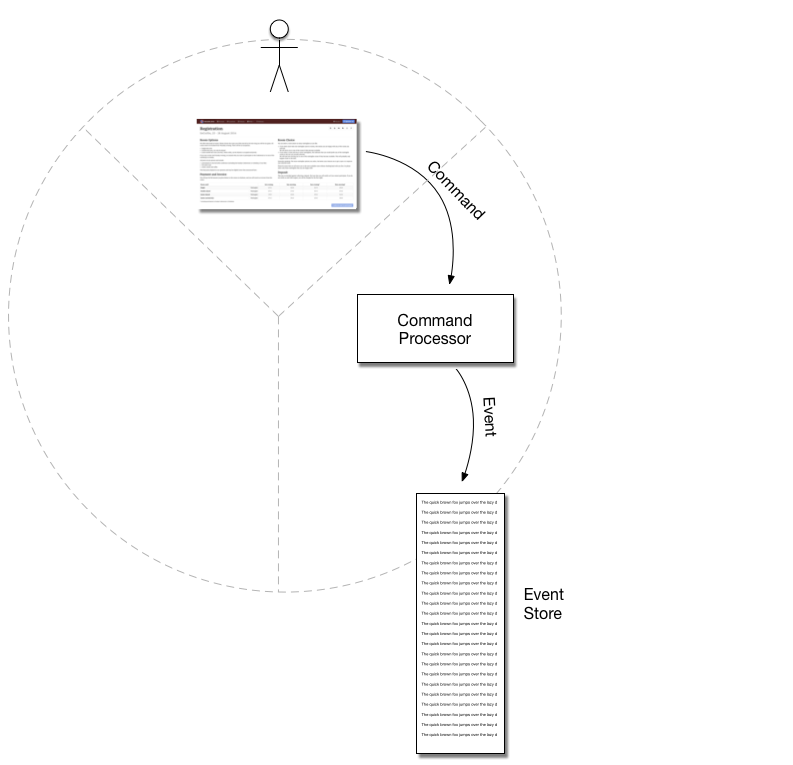
\includegraphics[width=.7\textwidth]{../EventSourcing2.png}
\end{onlyenv}

\begin{onlyenv}<3-4>
\begin{minipage}{.7\textwidth}
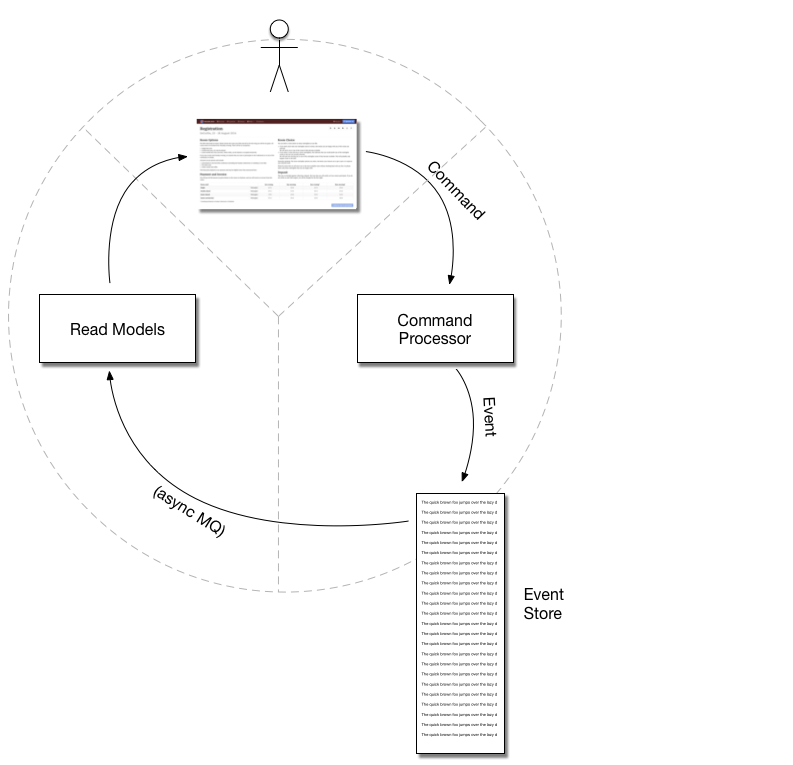
\includegraphics[width=\textwidth]{../EventSourcing3.png}
\end{minipage} \hfill
\end{onlyenv}
\begin{onlyenv}<3>
\begin{minipage}{0.25\textwidth}
\small
Set ticket count
\begin{itemize}
\item Ticket count set
\end{itemize}
\end{minipage}
\end{onlyenv}
\begin{onlyenv}<4>
\begin{minipage}{0.25\textwidth}
\small
Book ticket
\begin{itemize}
\item Ticket booked
\item Sold out
\item You already booked a ticket
\end{itemize}
\end{minipage}
\end{onlyenv}

\begin{onlyenv}<5>
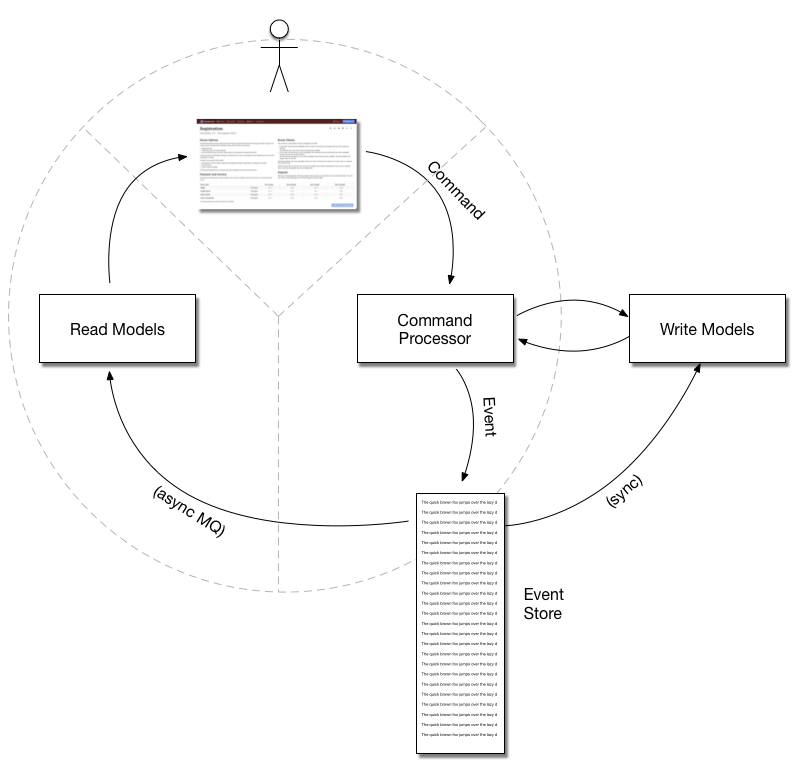
\includegraphics[width=.7\textwidth]{../EventSourcing4.png}
\end{onlyenv}

\end{frame}

%%%%%%%%%%%%%%%%%%%%%%%%%%%%%%%%%%%%%%%%%%%%%%%%%%
\begin{frame}[fragile]{Standard Event Sourcing Scenario}

\begin{itemize}
\item Event sourcing in application server
\item Incremental updates of event store, write models and read models
\item Write models must be updated synchronously
\item Read models can be updated asynchronously
\end{itemize}

\end{frame}

%%%%%%%%%%%%%%%%%%%%%%%%%%%%%%%%%%%%%%%%%%%%%%%%%%
\begin{frame}[fragile]{Event Sourcing in Node.js}

Let's understand how node.js works

\end{frame}

%%%%%%%%%%%%%%%%%%%%%%%%%%%%%%%%%%%%%%%%%%%%%%%%%%
\begin{frame}[fragile]{Node.js}

\begin{onlyenv}<1>
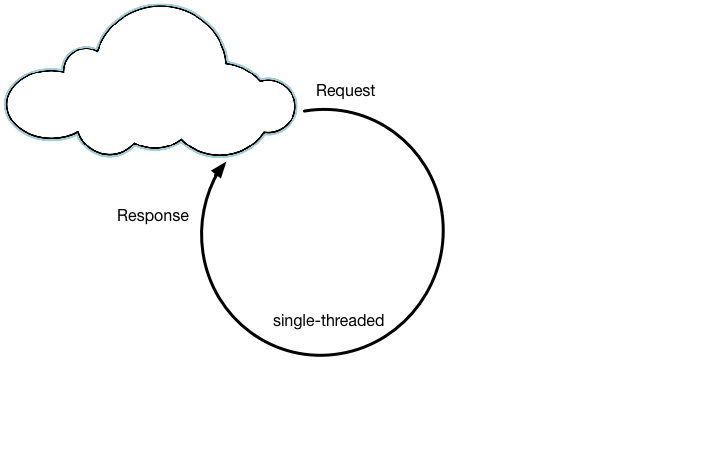
\includegraphics[width=.7\textwidth]{../Nodejs1.png}
\end{onlyenv}

\begin{onlyenv}<2>
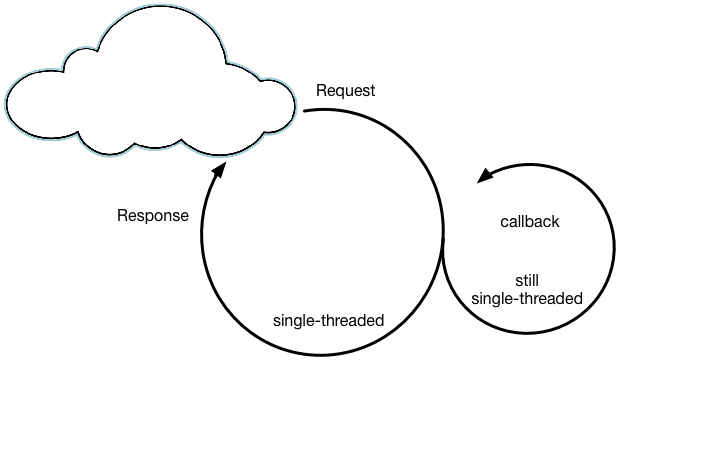
\includegraphics[width=.7\textwidth]{../Nodejs2.png}
\end{onlyenv}

\begin{onlyenv}<3>
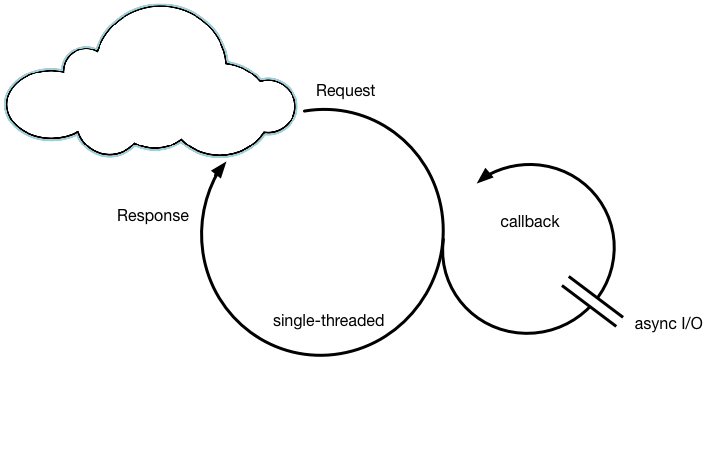
\includegraphics[width=.7\textwidth]{../Nodejs3.png}
\end{onlyenv}

\begin{onlyenv}<4>
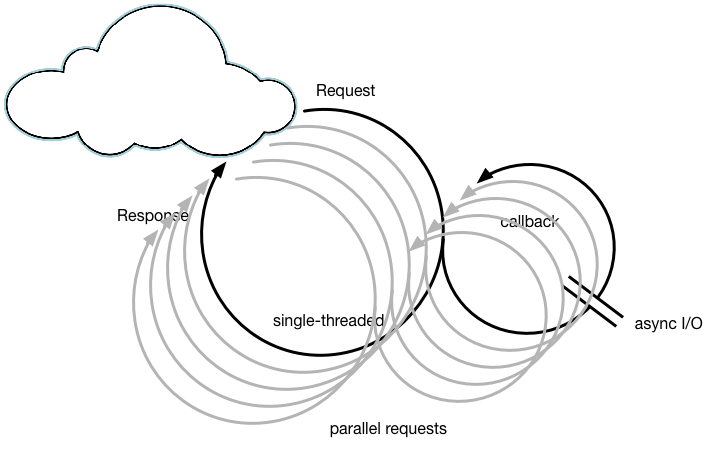
\includegraphics[width=.7\textwidth]{../Nodejs4.png}
\end{onlyenv}

\hfill 

\begin{tiny}
\makebox[\textwidth][r]{\url{http://blog.mixu.net/2011/02/01/understanding-the-node-js-event-loop/}}
\end{tiny}

\end{frame}

%%%%%%%%%%%%%%%%%%%%%%%%%%%%%%%%%%%%%%%%%%%%%%%%%%
%\begin{frame}[fragile]{}

%\end{frame}


%%%%%%%%%%%%%%%%%%%%%%%%%%%%%%%%%%%%%%%%%%%%%%%%%%
%%%%%%%%%%%%%%%%%%%%%%%%%%%%%%%%%%%%%%%%%%%%%%%%%%
%%%%%%%%%%%%%%%%%%%%%%%%%%%%%%%%%%%%%%%%%%%%%%%%%%
\begin{frame}[fragile]{}

Implementation in Node.js and Mongo-DB

\end{frame}

%%%%%%%%%%%%%%%%%%%%%%%%%%%%%%%%%%%%%%%%%%%%%%%%%%
\begin{frame}[fragile]{}

EventSourcing ohne globalen State

\end{frame}

%%%%%%%%%%%%%%%%%%%%%%%%%%%%%%%%%%%%%%%%%%%%%%%%%%
\begin{frame}[fragile]{}

Node: Single-Threaded, aber trotzdem ... (was?)

\end{frame}

%%%%%%%%%%%%%%%%%%%%%%%%%%%%%%%%%%%%%%%%%%%%%%%%%%
\begin{frame}[fragile]{}

Implementierung Optimistic Locking

\end{frame}

%%%%%%%%%%%%%%%%%%%%%%%%%%%%%%%%%%%%%%%%%%%%%%%%%%
\begin{frame}[fragile]{}

Implementierung Event Sourcing

\end{frame}

%%%%%%%%%%%%%%%%%%%%%%%%%%%%%%%%%%%%%%%%%%%%%%%%%%
\begin{frame}[fragile]{}

{
\LARGE

Outcome
}

\end{frame}

%%%%%%%%%%%%%%%%%%%%%%%%%%%%%%%%%%%%%%%%%%%%%%%%%%
\begin{frame}[fragile]{}

Registration began
                  
                  but nobody registered!
                  
\end{frame}

%%%%%%%%%%%%%%%%%%%%%%%%%%%%%%%%%%%%%%%%%%%%%%%%%%
\begin{frame}[fragile]{}

Ablauf skizzieren. 
                  
                  First user came in
                  reading from DB parallelized it
                  somebody else modified the DB
                  first user could not save
                  retry
                  same happened again, and again
                  
                  reading of read and write models was slow
                  so many other connections came through and modified DB
                  
                  self-propelling disaster
                  
\end{frame}

%%%%%%%%%%%%%%%%%%%%%%%%%%%%%%%%%%%%%%%%%%%%%%%%%%
\begin{frame}[fragile]{}

After 25 minutes, I shut down the server.
                  
                  Nobody had been able to register.
                  
\end{frame}

%%%%%%%%%%%%%%%%%%%%%%%%%%%%%%%%%%%%%%%%%%%%%%%%%%
\begin{frame}[fragile]{}

{
\LARGE

Improvements
}

\end{frame}

%%%%%%%%%%%%%%%%%%%%%%%%%%%%%%%%%%%%%%%%%%%%%%%%%%
\begin{frame}[fragile]{}

Analysis: Because of parallelization, it was impossible for one user to get through.
                  
                  We must control parallelization.
                  
\end{frame}

%%%%%%%%%%%%%%%%%%%%%%%%%%%%%%%%%%%%%%%%%%%%%%%%%%
\begin{frame}[fragile]{}

Nachteil: Jetzt ist keine Parallelisierung von Prozessen mehr möglich

\end{frame}


%%%%%%%%%%%%%%%%%%%%%%%%%%%%%%%%%%%%%%%%%%%%%%%%%%
\begin{frame}[fragile]{Nested Components}

\vspace{-2em}
\begin{lstlisting}{JavaScript}
export default class extends Component {
  render() {
    return (
      <div>
        <p>Nested Component with</p>
        <SimpleComponent />
      </div>
    ); }}
\end{lstlisting}

\vspace{-0.5em}

\begin{overlayarea}{\linewidth}{3cm}

\begin{onlyenv}<2-5,7->
\begin{lstlisting}{JavaScript}
const result = shallowRender(<NestedComponent />);
\end{lstlisting}
\end{onlyenv}

\begin{onlyenv}<2>
\vspace{-0.5em}
\begin{lstlisting}{JavaScript}
expect(JSON.stringify(result)).to.eql('{"type":"div","key":null,"ref":null,"props":{"children":' +
  '[{"type":"p","key":null,"ref":null,"props":{"children":"Nested Component with"},"_owner":null,"_store":{}},' +
  '{"key":null,"ref":null,"props":{},"_owner":null,"_store":{}}]},' +
  '"_owner":null,"_store":{}}');
\end{lstlisting}
\end{onlyenv}

\begin{onlyenv}<3-5>
\vspace{-0.5em}
\begin{lstlisting}{JavaScript}
expect(result.type).to.be('div');
expect(result.props.children.length).to.eql(2);
\end{lstlisting}
\end{onlyenv}

\begin{onlyenv}<4-5>
\vspace{-0.5em}
\begin{lstlisting}{JavaScript}
expect(result.props.children[0].type).to.eql('p');
\end{lstlisting}
\end{onlyenv}

\begin{onlyenv}<5>
\vspace{-0.5em}
\begin{lstlisting}{JavaScript}
expect(result.props.children[0].props.children).to.eql('Nested Component with');
\end{lstlisting}
\end{onlyenv}

\begin{onlyenv}<6>
\vspace{-0.5em}
\begin{center}

\textcolor{airbnb}{\textbf{\LARGE Enzyme}}
\end{center}
\end{onlyenv}

\begin{onlyenv}<7->
\vspace{-0.5em}
\begin{lstlisting}{JavaScript}
expect(JSON.stringify(result.props.children[1])).to.eql(
        '{"key":null,"ref":null,"props":{},"_owner":null,"_store":{}}');
\end{lstlisting}
\end{onlyenv}

\begin{onlyenv}<8->
\vspace{-0.5em}
\begin{lstlisting}{JavaScript}
import SimpleComponent from "../src/SimpleComponent";

expect(result.props.children[1].type).to.eql(SimpleComponent);
\end{lstlisting}
\end{onlyenv}

\end{overlayarea}


\end{frame}


%%%%%%%%%%%%%%%%%%%%%%%%%%%%%%%%%%%%%%%%%%%%%%%%%%
\begin{frame}{Thank you very much!}

        Code \& slides: \url{https://github.com/NicoleRauch/...}
        
        ~\\[1em]
        \begin{block}{Nicole Rauch}
        \begin{description}[Twitterxx]
                \item[E-Mail]  \href{mailto:info@nicole-rauch.de}{\texttt{info@nicole-rauch.de}}
                \item[Twitter] \href{http://twitter.com/NicoleRauch}{\texttt{@NicoleRauch}}
                \item[Web] \href{http://www.nicole-rauch.de}{\texttt{http://www.nicole-rauch.de}}
        \end{description}
        \end{block}
\end{frame}

